\documentclass{article}
\usepackage[utf8]{inputenc}
\usepackage{amsfonts}\usepackage{amssymb}\usepackage{amsmath}
\usepackage[top=2cm,left=1cm,right=1cm]{geometry}\usepackage{tikz}
\usepackage{gensymb}\usepackage{ragged2e}\usepackage{blindtext}\usepackage{polynom} \usepackage{graphicx}



\begin{document}
\begin{center}
    MAT110 ASSIGNMENT 1 [SET-28]\\[6pt]
    NAME: ANIKA ISLAM \\[6pt]
    ID:21101298 \\[6pt]
    SECTION:08
\end{center}
\newpage
\begin{figure}[htbp!]
    \centering
    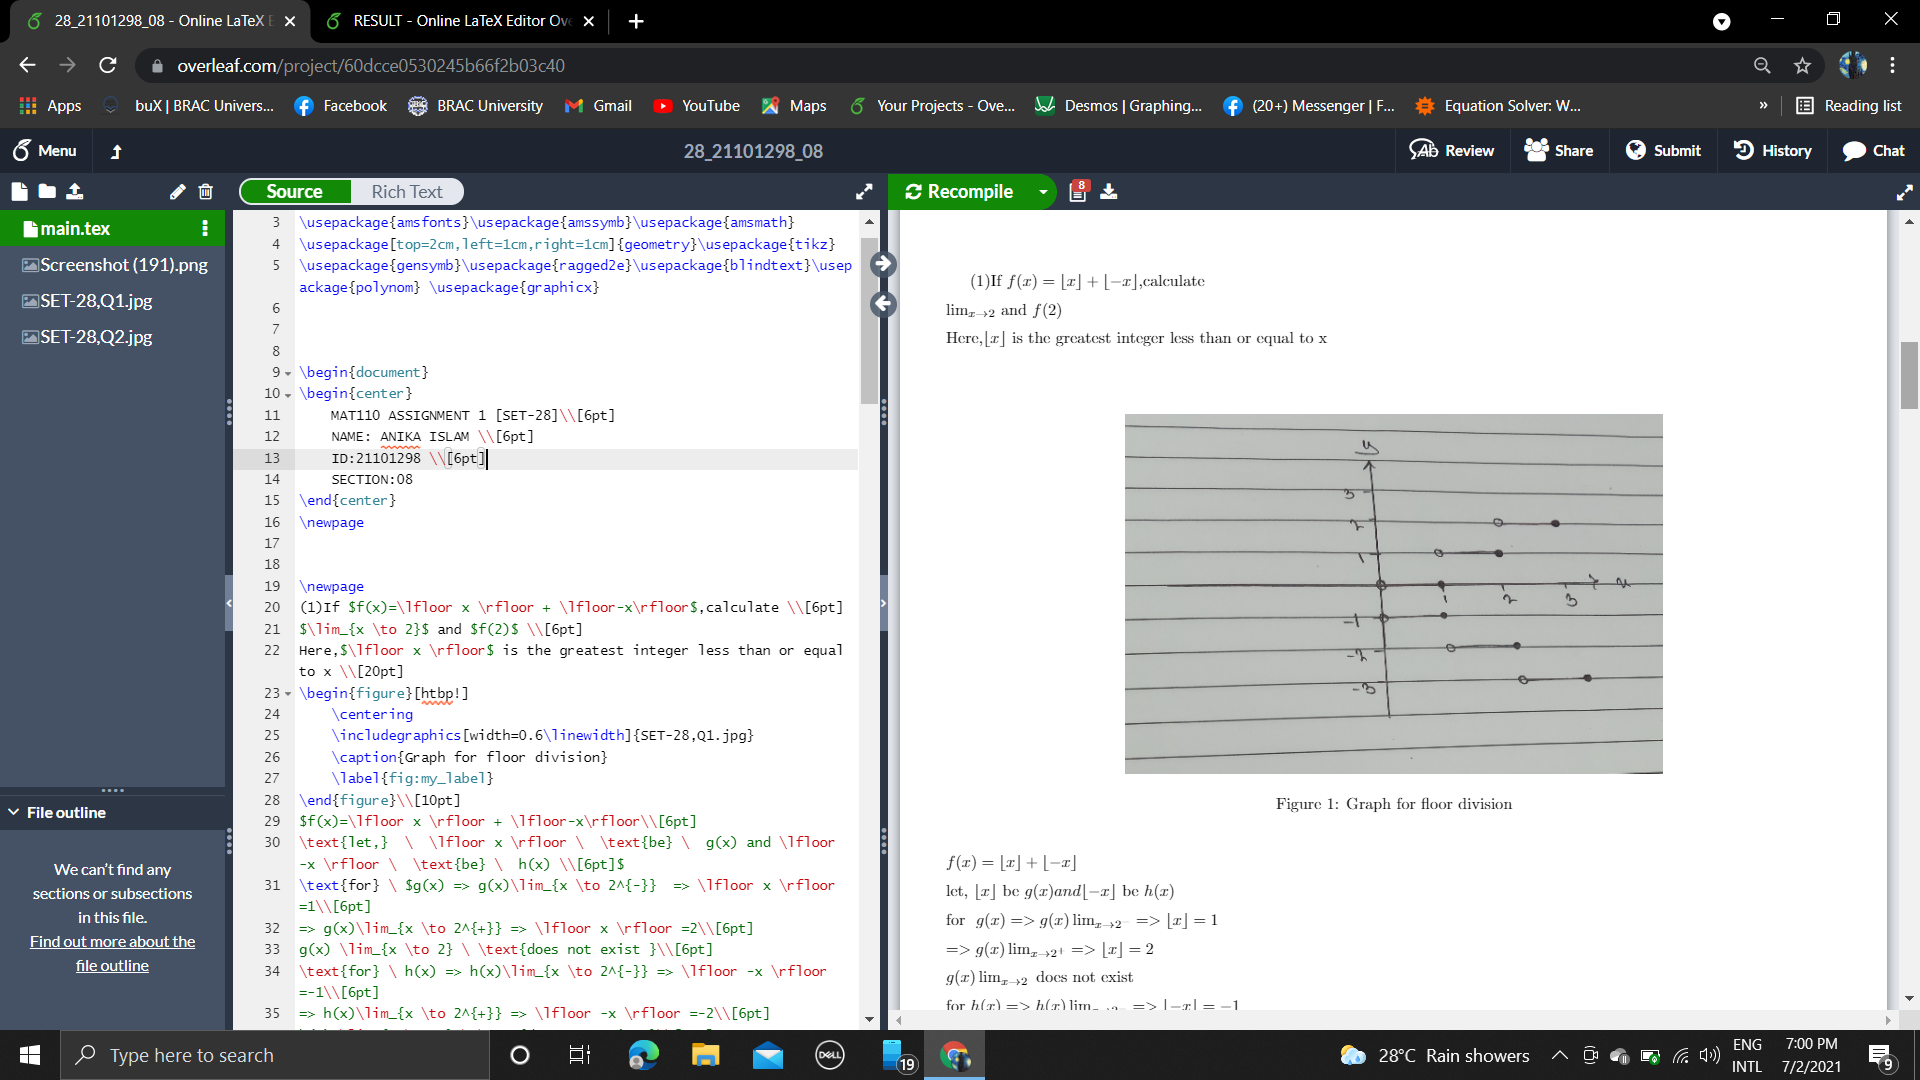
\includegraphics[width=1\linewidth]{Screenshot (205).png}
    \caption{Screenshoot of my Latex}
    \label{fig:my_label}
\end{figure}\newpage 
(1)If $f(x)=\lfloor x \rfloor + \lfloor-x\rfloor$,calculate \\[6pt]
$\lim_{x \to 2}$ and $f(2)$ \\[6pt]
Here,$\lfloor x \rfloor$ is the greatest integer less than or equal to x \\[20pt]
\begin{figure}[htbp!]
    \centering
    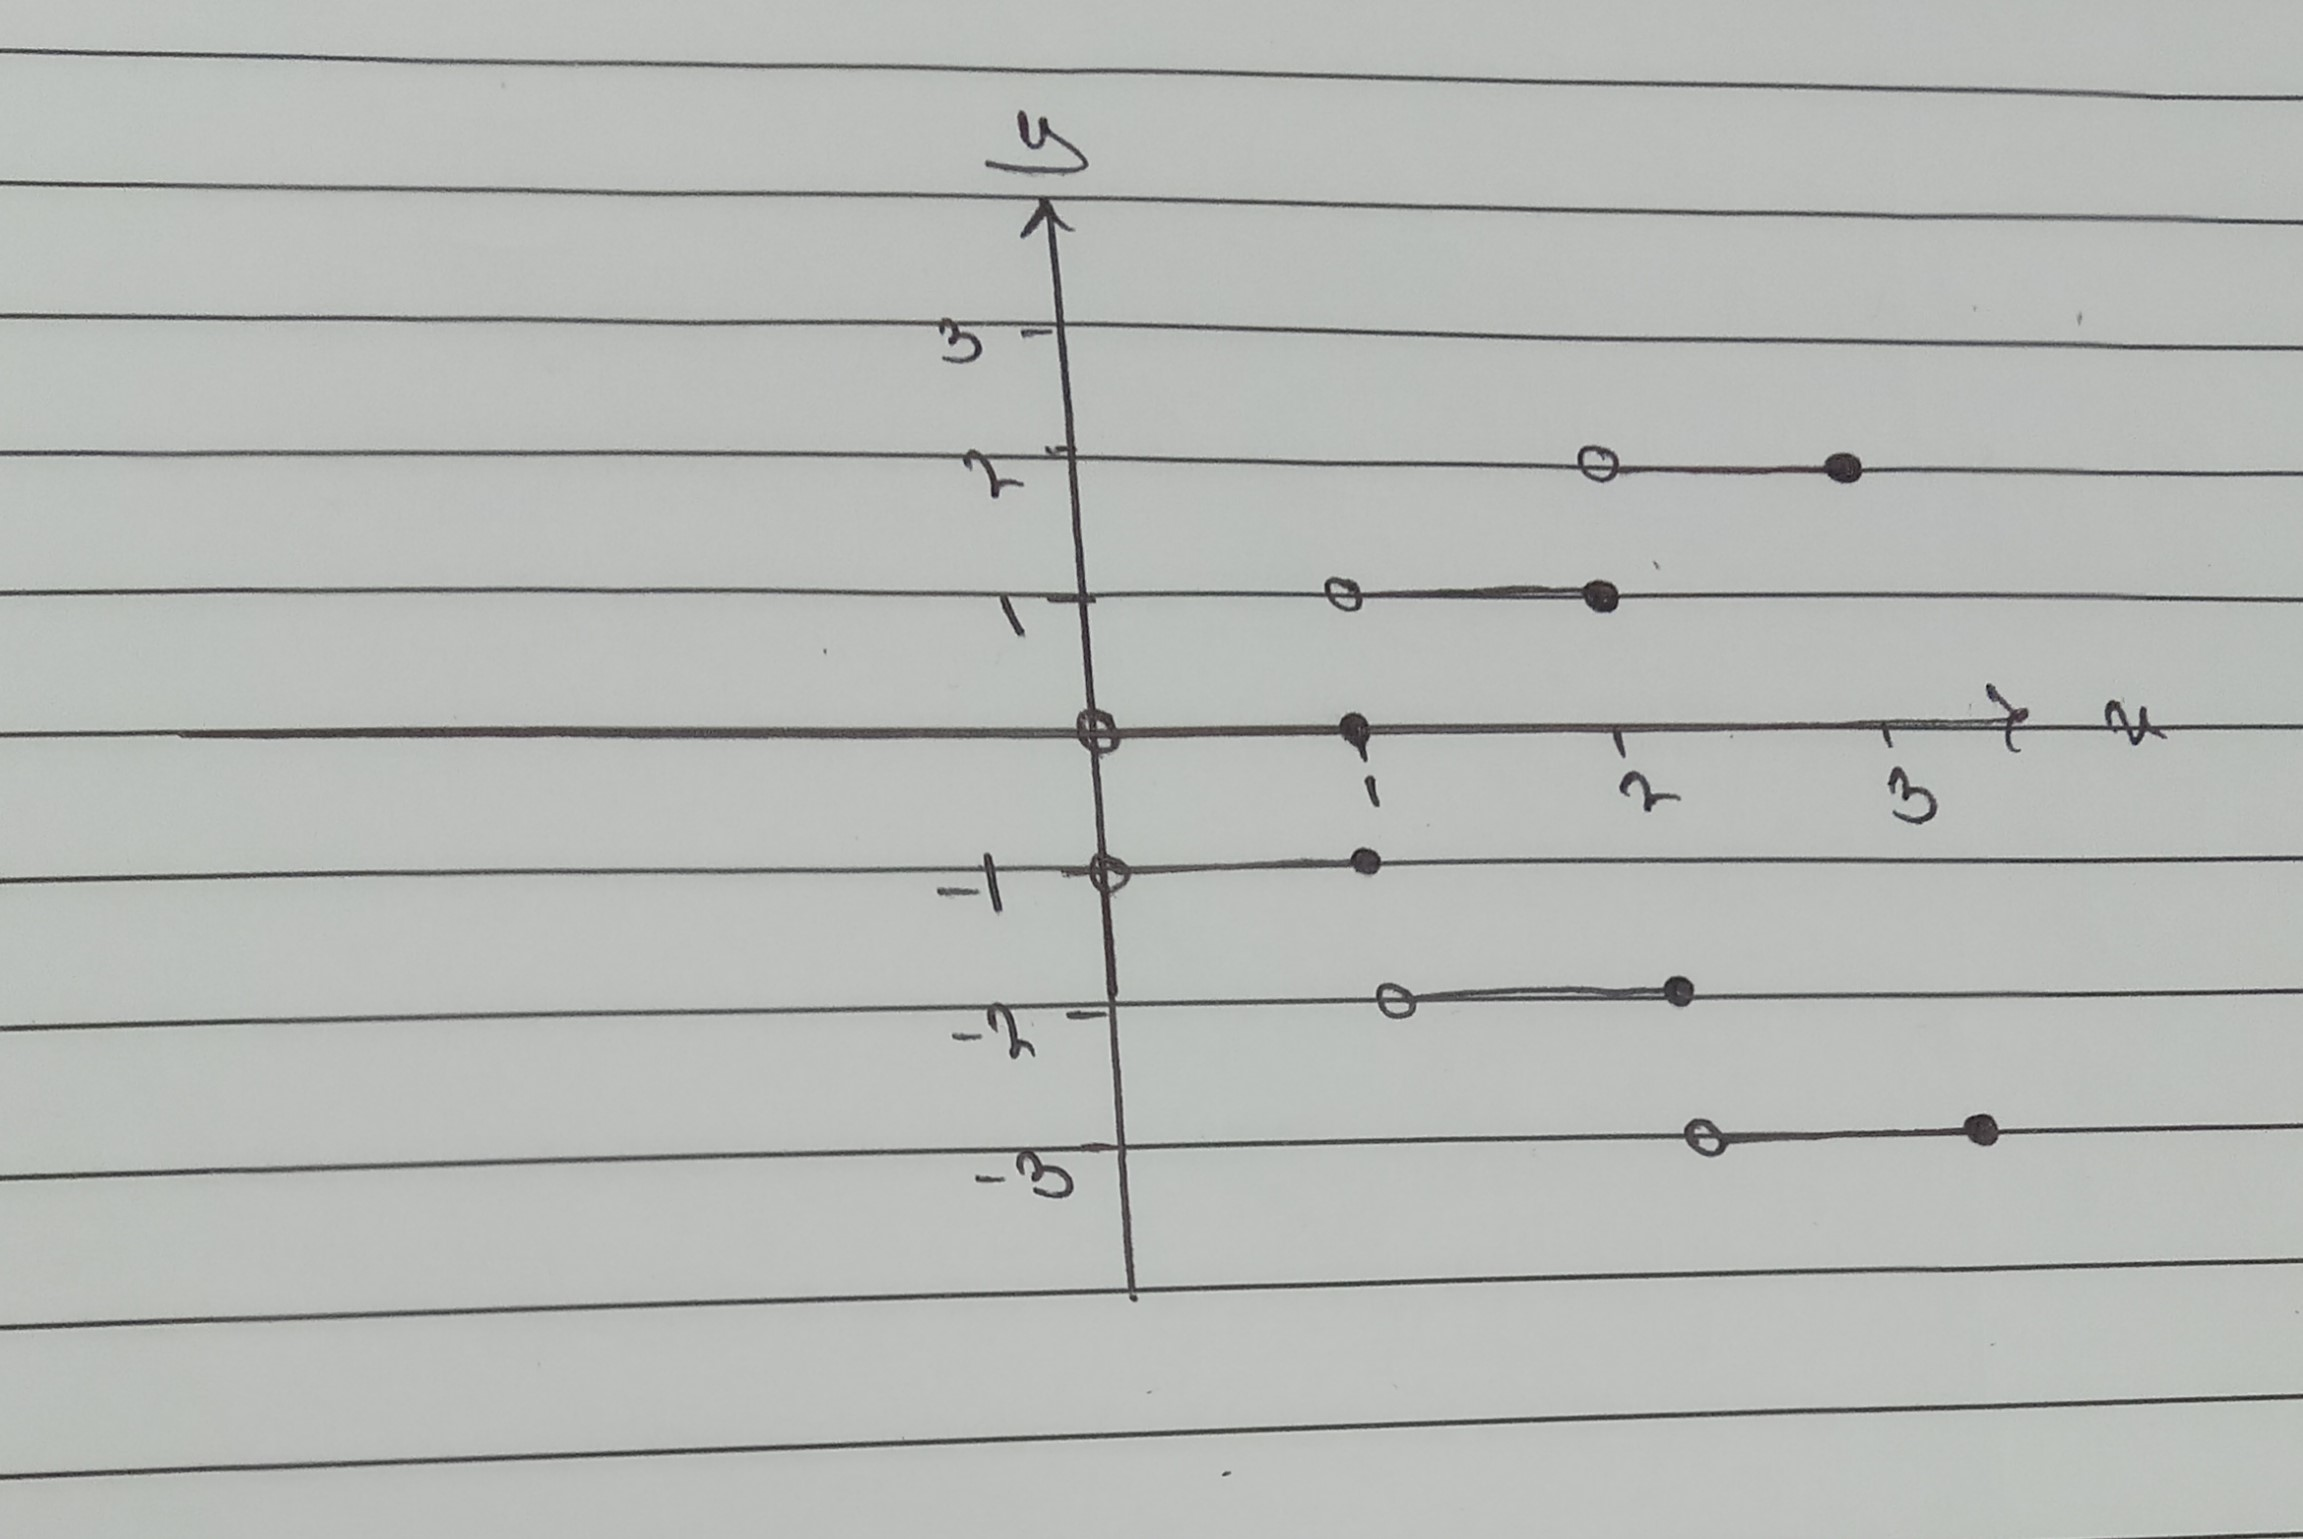
\includegraphics[width=0.6\linewidth]{SET-28,Q1.jpg}
    \caption{Sketch for floor division}
    \label{fig:my_label}
\end{figure}\\[10pt]
$f(x)=\lfloor x \rfloor + \lfloor-x\rfloor\\[6pt]
\text{let,}  \  \lfloor x \rfloor \  \text{be} \  g(x) and \lfloor -x \rfloor \  \text{be} \  h(x) \\[6pt]$
\text{for} \ $g(x) => g(x)\lim_{x \to 2^{-}}  => \lfloor x \rfloor =1\\[6pt]
=> g(x)\lim_{x \to 2^{+}} => \lfloor x \rfloor =2\\[6pt]
g(x) \lim_{x \to 2} \ \text{does not exist }\\[6pt]
\text{for} \ h(x) => h(x)\lim_{x \to 2^{-}} => \lfloor -x \rfloor =-1\\[6pt]
=> h(x)\lim_{x \to 2^{+}} => \lfloor -x \rfloor =-2\\[6pt]
h(x) \lim_{x \to 2} \ \text{does not exist }\\[6pt]
\text{for} \ f(x) => f(x)\lim_{x \to 2^{-}} => \lfloor x \rfloor + \lfloor -x \rfloor =2-3=-1\\[6pt]
=> f(x)\lim_{x \to 2^{+}} => \lfloor x \rfloor + \lfloor -x \rfloor =-2+1=-1\\[6pt]
f(x) \lim_{x \to 2} \ \text{ exist }\\[6pt]
f(x)\lim_{x \to 2}=\lfloor 2 \rfloor + \lfloor -2 \rfloor =0 \  \textbf{(answer)}\\[6pt]
f(2)=\lfloor 2 \rfloor + \lfloor -2\rfloor = 0\  \textbf{(answer)}$

\newpage
(2)Evaluate 
$$\lim_{x \to 0} \frac{|2x-1|-|2x+1|}{4} $$\\[20pt]
\begin{figure}[htbp!]
    \centering
    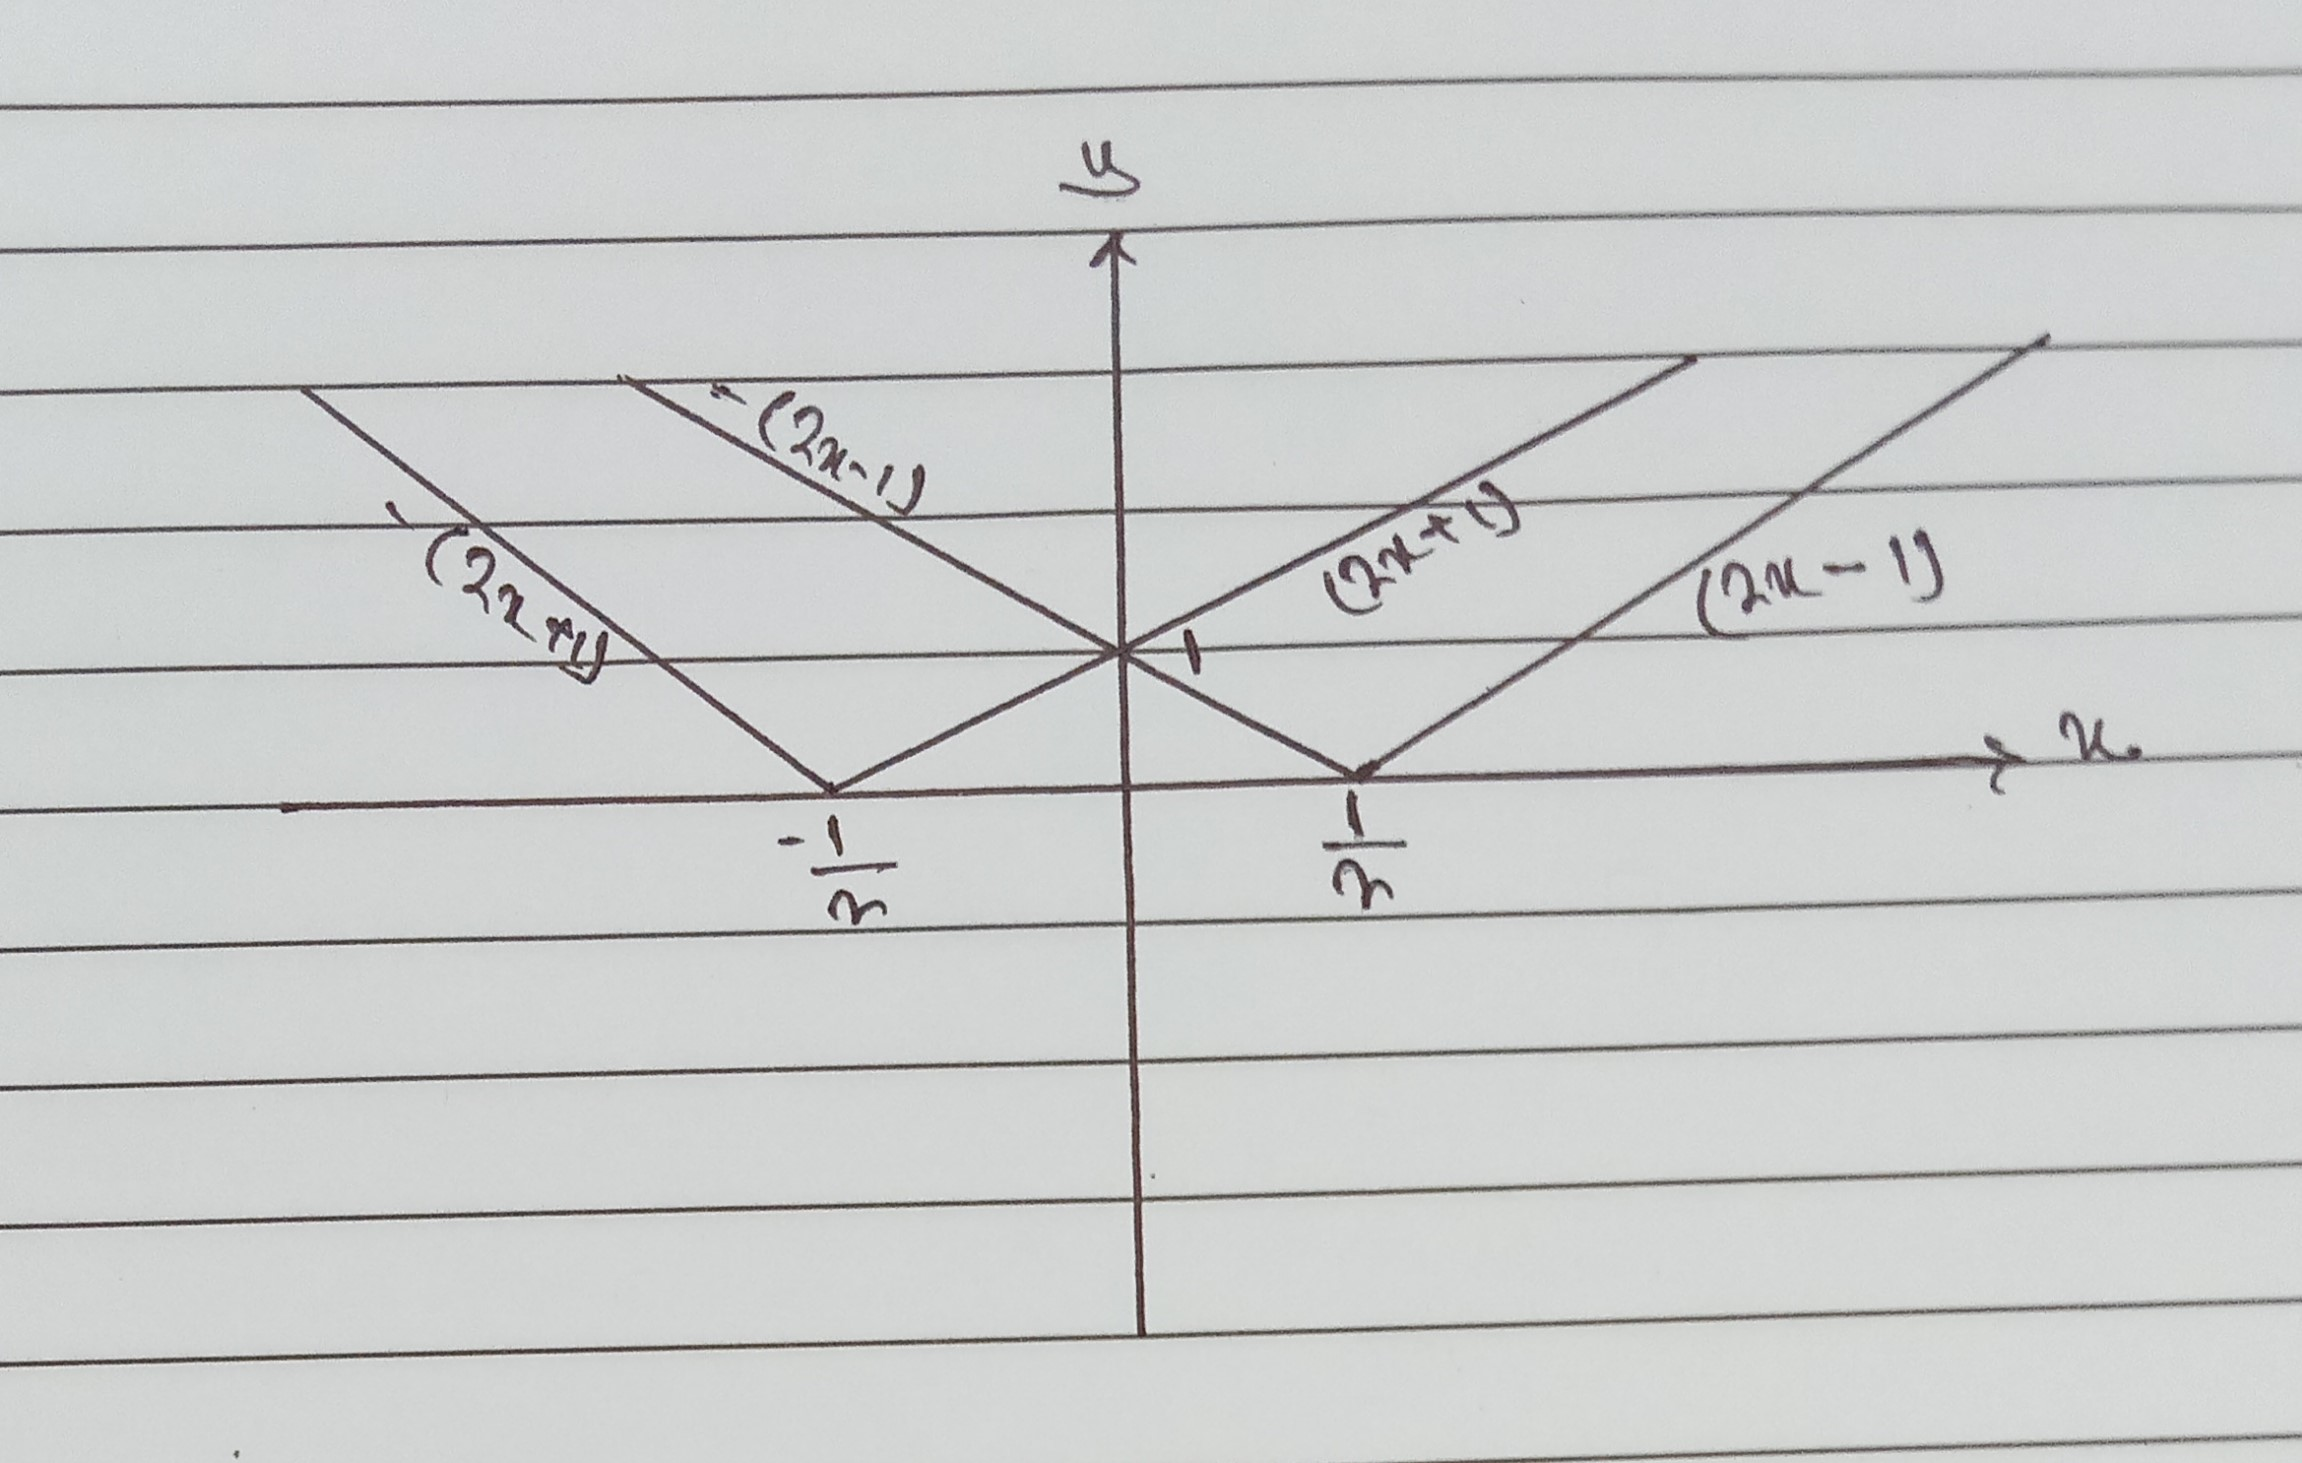
\includegraphics[width=0.6\linewidth]{SET-28,Q2.jpg}
    \caption{Sketch for $|2x-1| \  \text{and} \ |2x+1| $}
    \label{fig:my_label}
\end{figure}\\[20pt]
$\begin{cases}
2x-1 \ , \ x>\frac{1}{2}\\
-(2x-1) \ , \ x<\frac{1}{2}\\
2x+1 \ , \ x>-\frac{1}{2}\\
-(2x+1) \ , \ x<-\frac{1}{2}\\
\end{cases}$\\[10pt]
\text{for checking the right hand limit,}\\[6pt]
$\lim_{x \to 0^{+}}=-(2x-1)=1\\[6pt]
\text{for checking the left hand limit,}\\[6pt]
\lim_{x \to 0^{-}}=(2x+1)=1\\[6pt]
\lim{x \to 0} \ \text{limit exists}\\[6pt]
\lim_{x \to 0} \frac{|2x-0|-|2x+0|}{4} = \frac{0}{4} \\[6pt]
\lim_{x \to 0} \frac{|2x-0|-|2x+0|}{4} = 0 \  \textbf{(answer)}\\[20pt]
$
\newpage
(3)Find:
$$\lim_{x \to \infty} \frac{x^{2}(2+\sin^{2}x)}{x+100}$$\\[20pt]
$\lim_{x \to \infty} \frac{x^{2}(2+\sin^{2}x)}{x+100}\\[6pt]
=\lim_{x \to \infty} \frac{\frac{x^{2}(2+\sin^{2}x}{x^{2}}}{\frac{x+100}{x^{2}}}  \   [\text{dividing with}  \ x^{2}]\\[6pt]
=\lim_{x \to \infty} \frac{2+\sin^{2}x}{\frac{1}{x}+\frac{100}{x^{2}}}\\[6pt]
=\lim_{x \to \infty} \frac{2+\sin^{2}x}{x^{-1}+100x^{-2}}\\[6pt]
=\lim_{x \to \infty} \frac{2+\sin^{2}x}{x^{-1}+100x^{-2}}\\[6pt]
=\lim_{x \to \infty} \frac{2+\sin^{2}\infty}{\infty^{-1}+100\infty^{-2}}\\[6pt]
=\lim_{x \to \infty} \frac{2+0}{0+100(0)}\\[6pt]
=\lim_{x \to \infty} \frac{2}{0}\\[6pt]
\lim_{x \to \infty} \frac{x^{2}(2+\sin^{2}x)}{x+100}=\infty  \ \textbf{(answer)}\\[20pt]
$
\newpage
(4) Using L'Hospital's rule,find
$$\lim_{x \to \infty} x^{\frac{1}{x}}$$\\[20pt]
$\ln \lim_{x \to \infty}  \ln x^{\frac{1}{x}}\\[6pt]
= \ln \lim_{x \to \infty} \frac{1}{x}\ln x \\[6pt]
=\ln \lim_{x \to \infty} \frac{\ln x}{x}  \\[6pt]
=\ln \lim_{x \to \infty} \frac{\ln x}{x}  \\[6pt]
= \ln \lim_{x \to \infty} \frac{1}{x} \ln x \\[6pt]
=\lim_{x \to \infty} e^{\frac{1}{x}}\\[6pt]
=\lim_{x \to \infty} e^{\frac{1}{\infty}}\\[6pt]
=\lim_{x \to \infty} e^{0}\\[6pt]
=\lim_{x \to \infty} x^{\frac{1}{x}}=1  \  \textbf{(answer)}$

\newpage
(5) Using implicit differentiation, find $y',y''$ as functions of $x$ and $y$ \ , \ given
$$\sin x+\cos y = exp(4y)$$\\[20pt]
$\sin x+\cos y = exp(4y)\\[6pt]
=>\cos x - (\sin y )y'= (4exp(4y)) y' \\[6pt]
=>\cos x = y'(4exp(4y)+\sin y)\\[6pt]
=>y'=\frac{\cos x}{(4exp(4y)+\sin y)}\\[10pt]
=>y''=\frac{(4exp(4y)+\sin y)\frac{d}{dx}(\cos x)-(\cos x)\frac{d}{dx}(4exp(4y)+\sin y)}{(4exp(4y)+\sin y)^{2}}\\[6pt]
=>y''= \frac{(4exp(4y)+\sin y)(-\sin x)-(\cos x)((16exp(4y)+\cos y)y')}{(4exp(4y)+\sin y)^{2}}\\[6pt]
=>y''=\frac{(4exp(4y)+\sin y)(-\sin x)-(\cos x)(16exp(4y)+\cos y)\frac{\cos x}{(4exp(4y)+\cos y)}}{(4exp(4y)+\sin y)^{2}}\\[6pt]
=>y''=\frac{-\sin x(4exp(4y)+\sin y)^{2}-(\cos x)^{2}(16exp(4y)+\cos y)}{(4exp(4y))+\sin y)^{3}}  \ \textbf{(answer)}\\[6pt]
$
\newpage
(6) Differentiation $f(x)=\ln(\sin x - \cot x)$ \ with respect to $x$\\[20pt]
$f(x)=\ln(\sin x - \cot x)\\[6pt]
y=\ln u \ , \ u=\sin x - \cot x \\[6pt]
=>\frac{dy}{du}=\frac{1}{u}\\[6pt]
\text{differentiation of } \ \cot x \\[6pt]
=\frac{1}{\tan x}\\[6pt]
=\frac{(\tan x)\frac{d}{dx}(1)-(1)\frac{d}{dx}(\tan x)}{\tan^{2}x}\\[6pt]
=\frac{0-\sec^{2}x}{\tan^x}\\[6pt]
=-\frac{\frac{1}{\cos^{2}x}}{\frac{\sin^{2}x}{\cos^{2}x}}\\[6pt]
=-\frac{1}{\sin^{2}x}\\[6pt]
=-\csc^{2}x\\[6pt]
=>\frac{du}{dx}=\cos x + \csc^{2}x\\[6pt]
=>\frac{dy}{dx}=\frac{dy}{du}.\frac{du}{dx}\\[6pt]
=>\frac{dy}{dx}=\frac{1}{u}.\cos x + \csc^{2}x\\[6pt]
=>\frac{dy}{dx}=\frac{1}{\sin x - \cot x}.\cos x + \csc^{2}x\\[6pt]
=> \frac{dy}{dx}=\frac{\cos x + \csc^{2}x}{\sin x - \cot x}  \ \textbf{(answer)}\\[20pt]
$
\end{document}




\newpage 
1)American Airlines requires that the total outside dimensions (length+width+height)
of a checked bag not exceed 62 inches. Suppose you want to check a bag whose
height is same as its width. What is the largest volume bag of this shape that
you can check on an American Air Flight?\\[20pt]
$V=lwh \\[6pt]
\therefore w=h \\[6pt]
V=lw.w \\[6pt]
V=lw^{2}\\[6pt]
l + w + h = 62 \\[6pt]
l +w + w = 62 \\[6pt]
l = 62 - 2w \\[6pt]
V = lw^{2} = (62 - 2w)(w^{2}) = 62w^{2} - 2w^{3} \\[6pt]
\frac{dV}{dw} = 124w - 6w^{2} \\[6pt]
At stationary points, \frac{dV}{dw} = 0 \\[6pt]
124w - 6w^{2} = 0 \\[6pt]
w(124 - 6w) = 0 \\[6pt]
w = 0  \ , \   w = \frac{62}{3} \\[6pt]$
\begin{table}[htbp!]
    \centering
    \begin{tabular}{|c|c|c|c|c|} \hline
        intervals &  values & $\frac{dV}{dw}$ & sign of $\frac{dV}{dw}$  & conclusion \\ \hline
         $(-\infty \ , \ 0)$ & $0$ & $124w - 62w^{2}$ & $0 $ & inflection \\ \hline
         $(0 \ , \ \frac{62}{3})$ & $\frac{62}{3}$ & $124w - 62w^{2}$ & +ve & increasing \\ \hline
          $(\frac{62}{3} \ , \ \infty)$ & $\frac{65}{3}$ & $124w - 62w^{2}$ & -ve & decreasing \\ \hline
    \end{tabular}
    \caption{Table for $\frac{dV}{dw}$}
    \label{tab:my_label}
\end{table}\\[6pt]
$l = 62 - 2(\frac{62}{3}) => l = \frac{62}{3} \\[6pt]
V_{max} = lw^{2} = (\frac{62}{3})^{3} = \mathbf{8827 inches^{3}}
